\subsection*{Introduction to Algorithm Evaluation}
Evaluating maximum matching algorithms requires a thorough assessment of each solver's performance across different scenarios. This approach helps us not only identify which algorithms perform well in specific situations but also determine if there is a "best" algorithm that consistently outperforms others. However, performance can vary widely depending on the graph structure and the parameters of the problem. Some algorithms prioritize accuracy but may take longer to run, while approximation algorithms, though faster, may not always yield optimal results. To capture these differences, we evaluate each solver based on both speed and accuracy, enabling us to identify which solvers are most effective in particular contexts and to better understand their strengths and limitations.

Our first goal in evaluating maximum matching algorithms is to determine, "Which algorithm is the fastest?" Since there isn’t a single “best” algorithm, we can only compare their performance relative to each other. To do this, we began by “racing” the algorithms—running them across all test cases and recording their results. Initially, we analyzed these results by plotting the total number of tests against the time taken. As shown below in the graph, this approach revealed that some algorithms were faster on certain test cases, while others solved a larger number of cases overall. These variations made the graphs difficult to interpret and the results inconclusive. This led us to establish more refined evaluation criteria to better analyze each algorithm’s speed and accuracy.

\begin{figure}[h!]
    \centering
    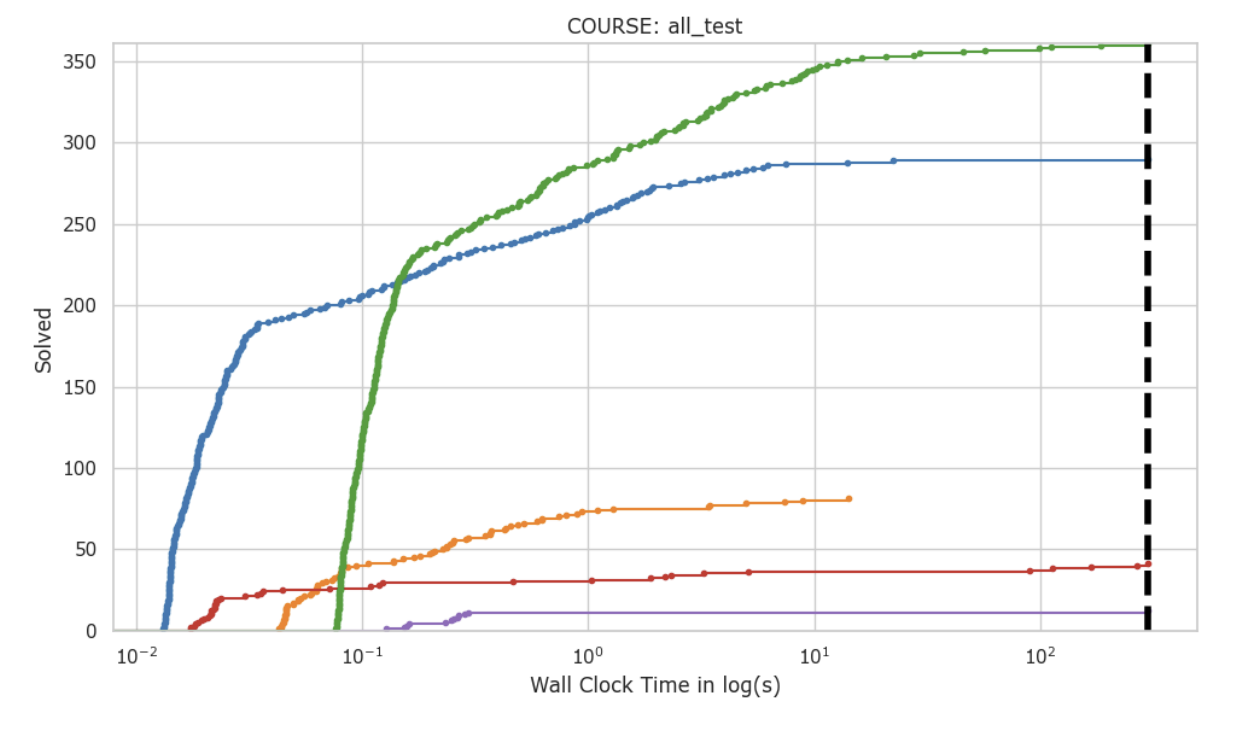
\includegraphics[width=0.6\textwidth]{all_test_course.png}
    \caption{Course: all\_test - Wall Clock Time vs Solved Instances}
    \label{fig:all_test_course}
\end{figure}

To better understand each algorithm’s performance across different categories, we organized the race into a set of courses. Each “course” is designed to test the algorithms in specific scenarios of the maximum matching problem, with a focus on different parameters like graph size, edge density, and matching characteristics. These courses simulate a variety of real-world and theoretical conditions, allowing us to isolate and examine distinct aspects of each algorithm’s behavior. By doing so, each course provides valuable insights into the relative effectiveness of the algorithms within that particular scenario.

Each course was developed to emphasize different graph characteristics based on the following parameters:

\begin{itemize}
    \item $d$: the number of partitions in the graph,
    \item $n$: the number of vertices,
    \item $m$: the number of edges, and
    \item $E$: the set of edges
    \item $M$: size of Maximum Matching
\end{itemize}

The courses that were studied are:
\begin{itemize}
    \item \textbf{Course 1: Perfect Matching} \\
    Tests solvers on graphs where every vertex can be matched.
    \item \textbf{Course 2: Random Matching (not perfect)} \\
    Uses graphs where perfect matching is not possible, highlighting algorithm behavior in imperfect matching situations.
    \item \textbf{Course 3: $\vert$Max-Matching$\vert$ in $[n/2,3n/4)$} \\
    Focuses on instances where the maximum matching is in the third quartile range.
    \item \textbf{Course 4: $\vert$Matching$\vert$ in $[3n/4, n-1]$} \\
    Instances where $\vert$Matching$\vert$ is in the fourth quartile, testing the solvers' efficiency on moderately large matching solutions.
    \item \textbf{Course 5: Large $n$ ($>1000$)} \\
    Evaluates solver performance on graphs with a large number of vertices, providing insight into scalability.
    \item \textbf{Course 6: Complete Graph} \\
    Examines algorithm efficiency on fully connected graphs.
    \item \textbf{Course 7: Large $m$ ($> \frac{n^d}{2}$) - Dense Graphs} \\
    Tests solvers on dense graphs where the number of edges $m$ exceeds half the maximum possible edges.
    \item \textbf{Course 8: Small $m$ ($< \frac{n^d}{2}$) - Sparse Graphs} \\
    Evaluates performance on sparse graphs, representing low-density structures.
    \item \textbf{Course 9: Easy problems with small $n$ and $m$ values} \\
    Provides a baseline with simpler problem instances with low vertex and edge counts.
\end{itemize}

Each course has specific values for the parameters listed above, allowing us to evaluate solver performance in different cases. By using a wide range of courses, we ensure that our evaluation is comprehensive and relevant to different types of maximum matching scenarios.\\
\\
Furthermore, we know that a bipartite matching problem runs in P whereas, for dimensions greater than 2, the problem is NP-hard. Thus, we split the algorithms into two categories: $d = 2$ and $d > 2$. This will better compare algorithms' performances by dividing them into P and NP problems.\\
\\
This evaluation framework is beneficial as it provides a deep understanding of solver performance. By analyzing algorithms under diverse conditions, we can make informed recommendations on which solver to use for different types of matching problems. The insights gained from these tests can guide the development of new, optimized algorithms for maximum matching problems, and help choose the best solver for specific use cases. The structure of courses and races allows for a robust comparison, ensuring that we can draw meaningful conclusions about each solver’s capabilities and limitations.